\chapter{Identification}
\section{Sputnik VAD}\label{Sputnik}
% graphic of Sputnik construction
The Sputnik VAD is an axial-flow blood pump, developed in a cooperative project of the National Research University of Electronic Technology, OJSC Zelenograd Innovation-Technology Center of Medical Equipment, FSBI "Academician V.I. Shumakov Federal Research Center of Transplantology and Artificial Organs", Ministry of Health of Russian Federation, DONA-M LLC and BIOSOFT-M LLC in 2009. \cite{Sputnik1}
\\This device is used for left ventricular assistance in patients with acute heart failure. The therapeutic objective in implantation of a Sputnik VAD is bridging to transplantation. The VAD is able to pump up to 10 liters of blood per minute with a continuous flow profile. The implantable pump weighs about $200\, g$, has a length of $81\, mm$ and a maximum diameter of $34\, mm$. It consists of a moving and a stationary part. The moving part, the impeller, a rotor with four blades, contains a permanent NdFeB-magnet, which is actuated by a brushless DC motor. The rotor spins clockwise with speed values between $4000-10000\, rpm$. An overview of the pump's specification is presented in \tablename~ \ref{tab:sput1}.
\begin{table}[ht]
  \centering
  \begin{tabular}{c|c}
    \toprule
    Blood flow  & 0-10 L/min \\
    Rotational speed & 4000-10000 rpm \\
    Length & 81 mm \\
    Diameter & 34 mm \\
    Weight & 200 g \\
    \bottomrule
\end{tabular}
  \caption[Specifications of Sputnik VAD]{Specifications of Sputnik VAD}
  \label{tab:sput1}
\end{table}
The stator is located inside a titanium housing with a $16\, mm$ diameter. The stationary part of the pump consists of a flow straightener with three stationary blades and a flow diffusor with three twisted blades. The flow straightener is located in front of the rotor and straightens the incoming blood flow into the rotor. Behind the rotor, blood is directed into the diffusor. %\cite{Sputnik1}
\figurename~ \ref{fig:sput_cross} depicts a cross-section of the Sputnik VAD and identifies its individual components.
The connection between the pump and the cardiovascular system is performed using in- and outflow cannulas, a felt ferule and vascular prosthesis which is sewed to the aorta. \cite{Sputnik1}
\begin{figure}[ht]
  \centering
  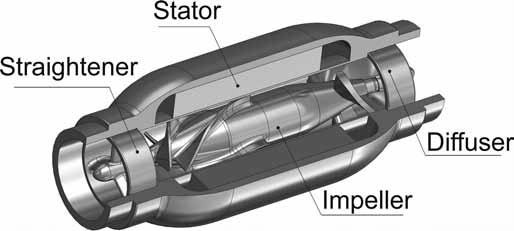
\includegraphics[width=0.6\textwidth]{images/sputnik_cross.png}
  \caption[Cross-section of Sputnik VAD \cite{Sputnik6}]{Cross-section of the Sputnik VAD \cite{Sputnik6}.}
  \label{fig:sput_cross}
\end{figure}
The Sputnik VAD is powered using two lithium-ion batteries, fully loaded providing enough energy for up to eight hours of system support. The maximum charging time for the batteries is less than five hours. During this time the batteries can either be exchanged by another set of batteries or the system can be powered through connection to an AC network. A microprocessor-based driving unit is used to regulate the pump speed, manage the power supply and store parameter data. It is connected percutaneously to the pump with an up to $170\, cm$ long and $5\, cm$ wide lead. \cite{Sputnik1}
\\During the practical part of this work the pump was controlled using the servo controller module ESCON 50/4 EC-S from maxon motor. This is a 4-quadrant pulse width modulation controller for controlling motors without Hall sensors.
%%%% ANSTEUERUNG ÜBER ESCON ERKLÄREN!!!

\section{Hardware in the Loop Test Bench}
For all measurements and tests performed during this thesis, a hardware in the loop (HiL) test bench of the Chair of Medical Information Technology at RWTH Aachen University was used. The test bench is implemented as a feedback controlled human circulatory system simulator. With the aid of the test rig, it is possible to test MCS systems under various physiological and pathological load patterns of the heart.
\begin{figure}[ht]
  \centering
  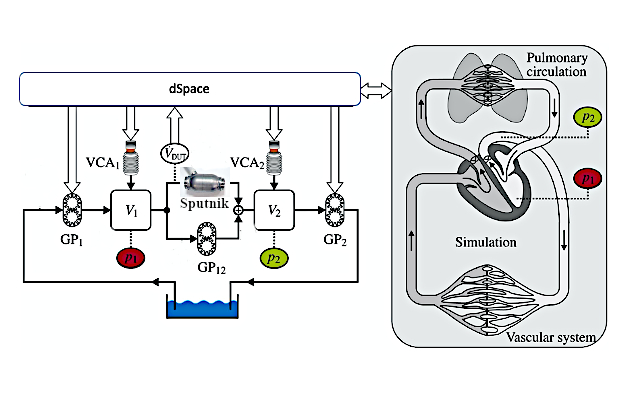
\includegraphics[width=\textwidth]{images/mock_loop.jpg}
  \caption[HiL test bench]{Structure of the HiL human ciculatory system simulator based on \cite{MCL}.}
  \label{fig:mock_loop}
\end{figure}
\\The structure of the mock circulatory loop (MCL) is depicted in \figurename~\ref{fig:mock_loop}. The boxes marked $V_{1}$ and $V_{2}$ are pressure compartments simulating the volume of the left ventricle and the aorta, respectively. Therefore, the pressure values of these compartments, referred to as $p_{1}$ and $p_{2}$, can be physiologically compared to the pressure values of the left ventricle and aorta. The MCL is actuated by three gear pumps ($GP_{1}$, $GP_{12}$ and $GP_{2}$) and two voice coil actuators ($VCA_{1}$ and $VCA_{2}$). The Sputnik VAD is connected to the pressure chambersin parallel, enabling tests similar to real use case. This way, the VAD can be subjected to similar pressure changes in the differential pressure between the aorta and ventricle as would be the case when used on the beating heart.
\\By controlling the MCL through a dSpace system (DS1103), pressure in the chambers can be adjusted in real time to simulate different cardiac dysfunctions. The dSpace system furthermore enables recording of reference signals presented to the MCL, as well as real time measurements. All recorded data can be exported formatted as Matlab matrices.
\\As the Sputnik VAD is not regularly included into the MCL setup, flow through the device can not be measured without further equipment. For this purpose the Transonic Systems Inc. T110 flow-meter is included in the setup. The flow sensor measurement is based on ultrasonic technology. The sensor probe, as presented in \figurename~\ref{fig:flow_meter_tube}, is adjusted onto the tube leading from the pressure chamber representing the left ventricle to the VAD. The flow-meter as well is connected to the dSpace system, enabling recording of the measured flow values. In \figurename~\ref{fig:mock_loop} these values are represented by $\dot{V}_{DUT}$.
\begin{figure}[ht]
  \centering
  \includegraphics[width=0.8\textwidth]{images/flow_meter.pdf}
  \caption[Sputnik VAD and flow-meter in HiL setup]{Sputnik VAD and flow-meter in HiL setup.}
  \label{fig:flow_meter_tube}
\end{figure}
\\The ESCON servo controller mentioned in chapter \ref{Sputnik} is also connected to the dSpace system. Using the digital input port of the controller a set value for regulation of the rotational speed can be transferred to the controller after setting the value in the system.
\\The dSpace system itself is controlled with the use of the program ControlDesk. This software provides the opportunity to include Matlab and Simulink source code. By this controllers designed under use of Simulink can directly be tested at the HiL test bench.

\section{System Identification}
%Vergleich Flüssigkeiten
%Vergleich Schlauchlängen
%Kennfeld
